\section{Implementation of the Experiment}
\label{sec:Durchführung}
To observe and record the Rubidum absoptionspectrum at the ende
of the experiment
serveral premeasurements with different setups are necessary.
% Used devices are two Photodiodes and
% of cause a diode laser
A dark room for the experiment is recommended to minize the
interfering light sources.

The used diode Laser

\subsection{Setup}
\label{subsec:setup}
The fist step is to determine the threshold current
of the diode laser.
Therefore a index card is placed in laser beam and the CCD Camera
is focused on the point where the card intercpets the beam.
The setup is displayed
in figure \ref{fig:setup1}.

\begin{figure}
  \centering
  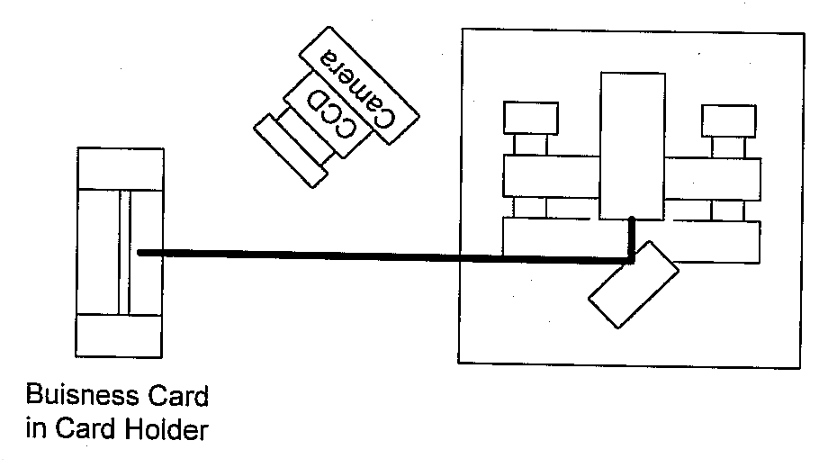
\includegraphics[width=0.7\textwidth]{setup1.png}
  \caption{Schematical setup to observe the threshold current of the diode laser.\cite{V61}}
  \label{fig:setup1}
\end{figure}
By increasing the current, starting at zero, the transition from
a normal LED to a laser diode be observed.
The threshold current is at the
transition point where the light spot becomes significant brighter.
% The thresholf current can verrigert werden durch
%( irgendwas mit den Rädchen)

After the threshold current is determined the
index card is removed and
the Rubidum Absorption Cell
is placed in the Laserbeam instead.
A Schematical setup is shown in figure \ref{fig:setup2}
The Camera is now
focus on the Absorption Cell and
the Diode is operated above the threshold current.

\begin{figure}
  \centering
  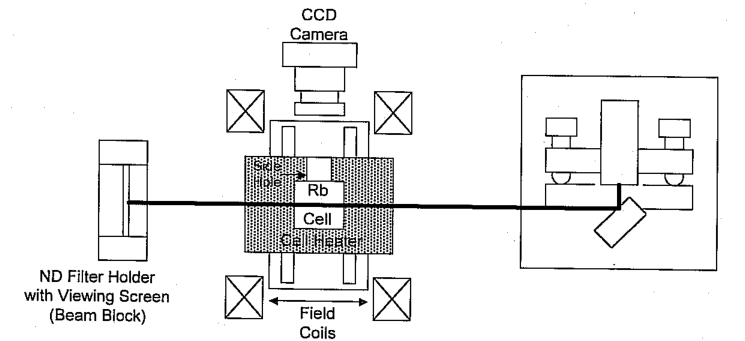
\includegraphics[width=0.7\textwidth]{setup2.png}
  \caption{Schematical setup to observe the Rubidium Florescence.\cite{V61}}
  \label{fig:setup2}
\end{figure}

 The



\begin{figure}
  \centering
  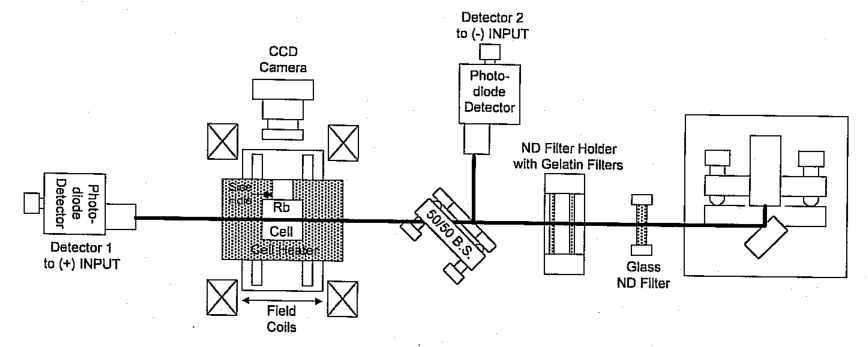
\includegraphics[width=0.7\textwidth]{setup3.png}
  \caption{Schematical setup to observe the Rubidium absoptionspectrum.\cite{V61}}
  \label{fig:setup3}
\end{figure}



\subsection{Procedure}
\label{subsec:procedure}
